\documentclass[12pt]{article}
\usepackage{amsfonts, amsmath, amsthm, amstext, amssymb}
\usepackage{mathtools}
\usepackage{nccmath}
\usepackage{graphicx}
\usepackage{hyperref}
\usepackage{blindtext}
\usepackage{wrapfig}

\marginparwidth 0pt
\oddsidemargin -1 truecm
\evensidemargin  0pt
\marginparsep 0pt
\topmargin -2.6truecm
\linespread{1}
\textheight 24.5truecm
\textwidth 18.4 truecm
\newenvironment{remark}{\noindent{\bf Remark }}{\vspace{0mm}}
\newenvironment{remarks}{\noindent{\bf Remarks }}{\vspace{0mm}}
\newenvironment{question}{\noindent{\bf Question }}{\vspace{0mm}}
\newenvironment{questions}{\noindent{\bf Questions }}{\vspace{0mm}}
\newenvironment{note}{\noindent{\bf Note }}{\vspace{0mm}}
\newenvironment{summary}{\noindent{\bf Summary }}{\vspace{0mm}}
\newenvironment{back}{\noindent{\bf Background}}{\vspace{0mm}}
\newenvironment{conclude}{\noindent{\bf Conclusion}}{\vspace{0mm}}
\newenvironment{concludes}{\noindent{\bf Conclusions}}{\vspace{0mm}}
\newenvironment{dill}{\noindent{\bf Description of Dill's model}}{\vspace{0mm}}
\newenvironment{maths}{\noindent{\bf Mathematics needed}}{\vspace{0mm}}
\newenvironment{object}{\noindent{\bf Objective}}{\vspace{0mm}}
\newenvironment{notes}{\noindent{\bf Notes }}{\vspace{0mm}}
\newenvironment{theorem}{\noindent{\bf Theorem }}{\vspace{0mm}}
\newenvironment{example}{\noindent{\bf Example }}{\vspace{0mm}}
\newenvironment{examples}{\noindent{\bf Examples }}{\vspace{0mm}}
\newenvironment{lemma}{\noindent{\bf Lemma }}{\vspace{0mm}}
\newenvironment{solution}{\noindent{\it Solution}}{\vspace{2mm}}
\newcommand{\QED}{\fbox{}}

\graphicspath{{converted_graphics/}}
\begin{document}
\baselineskip 18 pt
\begin{center}
{\bf \Large LANG1003I Academic Blog 1\\New Way of Learning}
\end{center}
\vspace{0.3cm}
Written on March 8, 2022 by KOO Kin Nam\\
\begin{wrapfigure}{r}{3in}
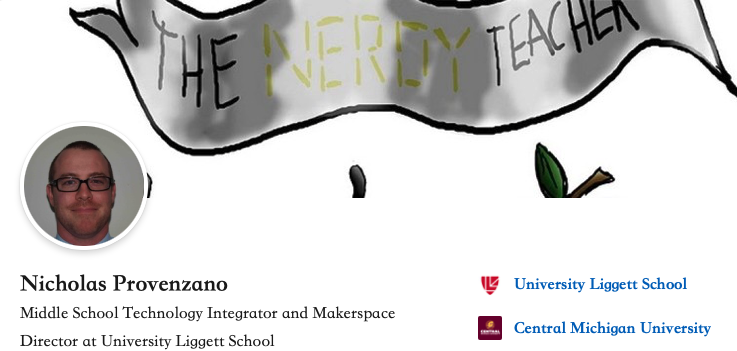
\includegraphics[scale = 0.3]{Photo2}
\caption[Yeah:]{}
\end{wrapfigure}

\blindtext
The article, “A short guide to Genius Hour makerspaces,” by Cheska Robinson discusses how to combine the concept of genius hour and makerspaces. Moreover, she also illustrates some recommendations on what teachers should do during the genius hour.  According to Robinson(2018), she stated that teachers can set up a makerspaces, which is a physical location for students to learn how to use new tools and create anything they want, and let students spend around a few “genius hours” a week to construct a project. Furthermore, she provided some tips for teachers such as getting the lay of the land, giving students ownership and showcasing student work.

Some of the sources used in the article are reliable, such as the author cited the definition of genius hour from a book “The Genius Hour Guidebook: Fostering Passion, Wonder, and Inquiry in the Classroom,” written by Denise Krebs, who is a grade 5 educator and graduated in Arizona State University and California State University, Long Beach. Moreover, when it comes to the advice for a genius hour makerspace, Robinson cited the suggestions from Nicholas Provenzano, a middle school technology integrator and makerspace director at University Liggett School. These show that the sources used by the writer are dependable. 


\includegraphics[scale = 0.3]{Photo1}Profolio of Denise Krebs in \href{https://about.me/mrsdkrebs}{about.me}\\


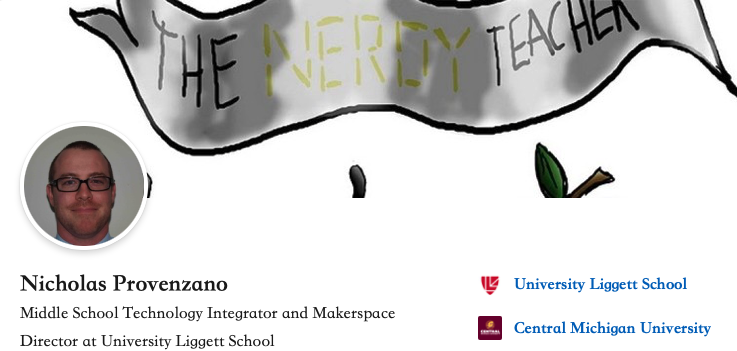
\includegraphics[scale = 0.3]{Photo2}
Profolio of Nicholas Provenzano in \href{https://www.linkedin.com/in/thenerdyteacher}{LinkedIn}\\

Besides, some of the instructions given by the writer are feasible to enhance the effectiveness of genius hour makerspace, such as having an endgame in mind. Most of us are good at starting a project, however, not many of the projects can be finished in the end. Students have to bear in mind that once they start a project of their own, they have the responsibility to complete it. 

Furthermore, it is good for the writer to combine genius hour and makerspace due to their similarity. Genius hour is a concept for students to have an in-class time to explore whatever they want while makerspace gives them a physical location to make their projects come true. They can learn new things and practice what they really like.

\begin{wrapfigure}{r}{3in}
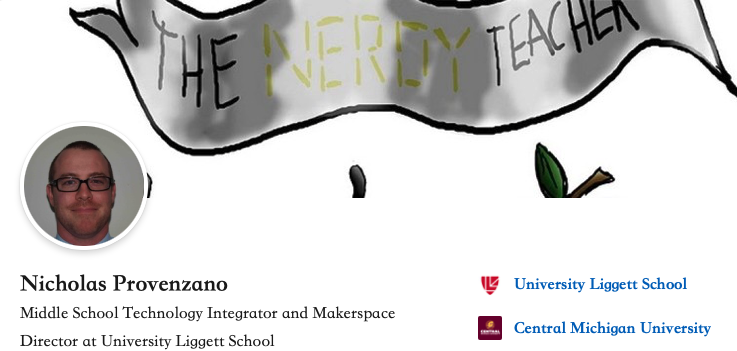
\includegraphics[scale = 0.3]{Photo2}
\end{wrapfigure}

All in all,  “A short guide to Genius Hour makerspaces,” gives the reader a practical method on how genius hour actually works. Not only illustrating the concept about spending hours for students to explore what they want, but also giving them an opportunity to finish a hands-on project.






\end{document}